\section{Varying Cepstrum Coefficients}
While including thirteen cepstrum coefficients in each feature has produced promising results, there may still be room for improvement by adding additional coefficients. We created a new data set with twenty-five coefficients in each feature. Three ten fold validation trials were conducted in the same manner as experiment II, with thirteen, nineteen, and all twenty-fave coefficients used as input, respectively. When all of them are not included in each feature, the coefficients are taken starting from the cepstrum with the lowest quefrency. We report the AUC score for each model using their soft-majority predictions.

\begin{table}[h]
\centering
\caption{Experimental results}
\begin{tabular}{|l|c|c|c|}
\hline
\multicolumn{1}{|c|}{}      &   13         &   19         &     25           \\ \hline
LSTM-1                      &   84.2     &   90.1     &     81.7       \\ \hline
LSTM-2                      &   79.1     &   88.2     &     87.1       \\ \hline
Bi-LSTM-1                   &   84.9     &   88.4     &     90.4       \\ \hline
\end{tabular}
\label{tab-results}
\end{table}

\begin{figure*}[t]
    \centering
    \begin{subfigure}[b]{0.4\textwidth}
        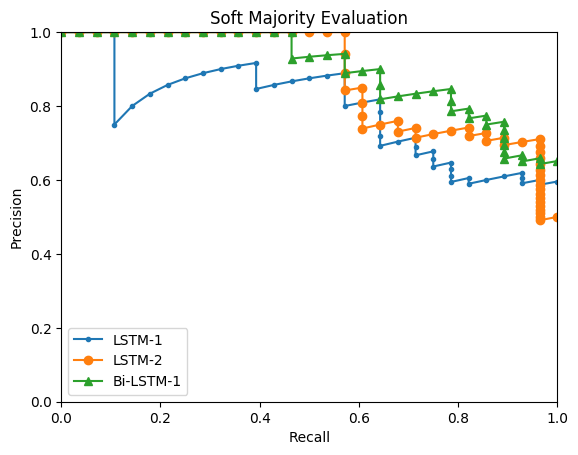
\includegraphics[width=\textwidth]{25cep-sm-pr.png}
        \caption{}
        \label{rfidtest_xaxis}
    \end{subfigure}
    \begin{subfigure}[b]{0.4\textwidth}
        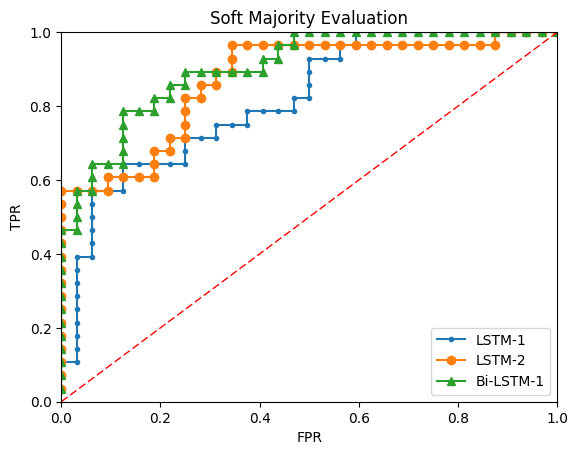
\includegraphics[width=\textwidth]{25cep-sm-roc.png}
        \caption{}
        \label{rfidtest_yaxis}
    \end{subfigure}
    \begin{subfigure}[b]{0.4\textwidth}
        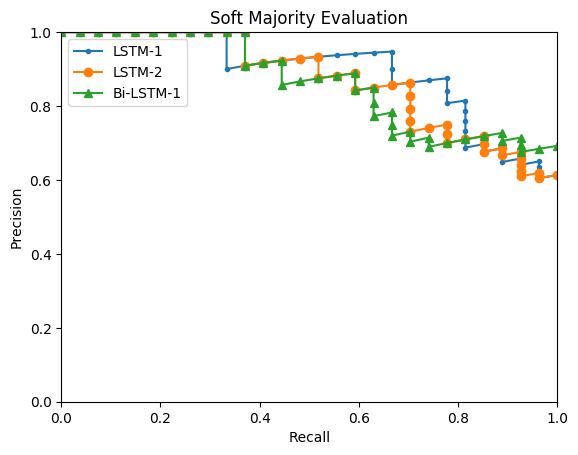
\includegraphics[width=\textwidth]{19cep-sm-pr.png}
        \caption{}
        \label{rfidtest_zaxis}
    \end{subfigure}
    \begin{subfigure}[b]{0.4\textwidth}
        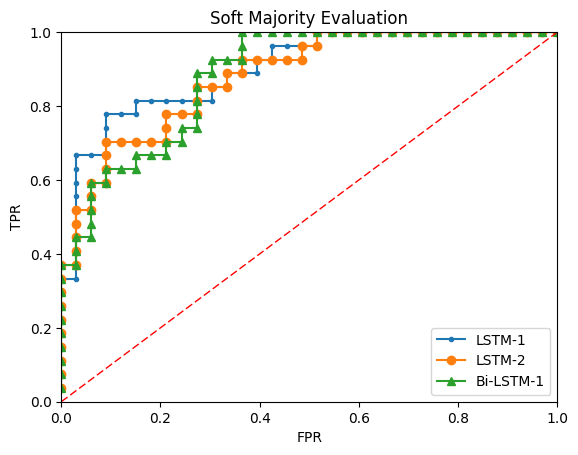
\includegraphics[width=\textwidth]{19cep-sm-roc.png}
        \caption{}
        \label{rfidtest_zaxis}
    \end{subfigure}
    \caption[]{}
    \label{rfidtag_testing}
\end{figure*}

Figure \ref{curves} I need to consolidate this into two graphs, an ROC and PR curve with all six models each.  

The standard thirteen coefficient input produced familiar results, but adding additional information to each feature lead to improved performance in some cases. Interestingly, $LSTM-1$ performed almost as well as $Bi-LSTM-1$ with size nineteen and twenty-five inputs, respectively. However, it seems the opposite is untrue, as $LSTM-1$'s performance decreases when given all of the coefficients as input. Considering it is the smallest model, in terms of parameters, it may be due to a lack of capacity. In general, it seems the models of sufficient size can take advantage of the extra coefficients. 

